%%%%%%%%%%%%%%%%%%%%%%%%%%%%%%%%%%%%%%%%%%%%%%%%%%%%%%%%%%%%%%%%%%%%%%
% TEMPLATE LaTeX – PAPER (STREAMLINED VARIANT)
% Versão: Paper para submissões de 6-10 páginas
% Descrição: Variante simplificada para artigos de conferência/periódico
%
% Dicas:
%  - Edite metadados em config/paper-config.tex
%  - Use [colchetes] para placeholders (renderizam bem no PDF)
%  - Insira figuras com \includegraphics e rotule com fig:, tab:, sec:, eq:
%  - Estrutura mínima: apenas capítulos essenciais
%  - Bibliografia: thebibliography (padrão simples)
%%%%%%%%%%%%%%%%%%%%%%%%%%%%%%%%%%%%%%%%%%%%%%%%%%%%%%%%%%%%%%%%%%%%%%

\documentclass[12pt]{article}

% =================================================================
% CONFIGURAÇÕES CENTRALIZADAS
% =================================================================
% =================================================================
% CONFIGURAÇÕES DO TEMPLATE - PAPER VARIANT
% Variant streamlined for 6-10 page conference/journal submissions.
% Como usar:
%  - Preencha os placeholders abaixo (título, autor, etc.)
%  - Adicione/remova pacotes conforme a necessidade do seu trabalho
%  - Mantenha overrides aqui, sem editar config/sbc-template.sty
% =================================================================

% Pacotes essenciais
\usepackage{config/sbc-template}
\usepackage[T1]{fontenc}   % melhor hifenização/acentuação com pdflatex
\usepackage[utf8]{inputenc}
\usepackage{microtype}     % microtipografia (kerning/hifenização)
\usepackage[english,brazil]{babel} % idiomas: en + pt-BR
\usepackage{csquotes}      % citações tipográficas
\usepackage{graphicx,url}
\graphicspath{{assets/}}   % pasta padrão para imagens

% Pacotes adicionais (essenciais para papers)
\usepackage{listings}           % listagens de código
\usepackage{xcolor}             % cores (necessário para listings)
\usepackage{amsmath,amssymb}    % matemática
\usepackage{booktabs}           % tabelas profissionais (\toprule, etc.)
\usepackage{hyperref}           % hyperlinks

% Estilo de código (exemplo; ajuste ou remova)
\definecolor{codegray}{RGB}{248,248,248}
\lstdefinestyle{code}{
    backgroundcolor=\color{codegray},
    basicstyle=\footnotesize\ttfamily,
    numbers=left,
    numbersep=5pt,
    frame=single,
}

% Hyperlinks (preenche metadados do PDF)
\hypersetup{
    colorlinks=true,
    linkcolor=black,
    urlcolor=blue,
    citecolor=blue,
    pdftitle={Test Project},
    pdfauthor={Test Author},
}

% Comandos de placeholders (consumidos em \title, \author e \address)
\newcommand{\DocumentTitle}{Test Project}
\newcommand{\AuthorName}{Test Author}
\newcommand{\AuthorInstitution}{Test Uni}
\newcommand{\AuthorLocation}{Test City}
\newcommand{\AuthorEmail}{test@example.com}

% Metadados padrão (para projetos que usam este arquivo como entrada principal)
\title{\DocumentTitle}
\author{\AuthorName\inst{1}}
\address{\AuthorInstitution\\
  \AuthorLocation\\
  \email{\AuthorEmail}
}

% Configurações gerais
\sloppy
\setlength{\parskip}{6pt}


% =================================================================
% INÍCIO DO DOCUMENTO
% =================================================================
\begin{document}

\maketitle

% =================================================================
% RESUMOS E ABSTRACTS
% =================================================================
% =================================================================
% ABSTRACT (INGLÊS)
% =================================================================
% Dicas: 150–250 palavras, sem citações ou fórmulas; voz ativa.
\begin{abstract}
  [Write the abstract in English here. Summarize the problem, method, results, and contributions in 150–250 words. Avoid citations and formulas.]
\end{abstract}

% =================================================================
% RESUMO (PORTUGUÊS)
% =================================================================
% Dicas: 150–250 palavras, sem citações; equivalência com o Abstract.
\begin{resumo}
  [Escreva o resumo em português aqui. Resuma o problema, método, resultados e contribuições em 150–250 palavras. Evite citações e fórmulas.]
\end{resumo}


% =================================================================
% CAPÍTULOS PRINCIPAIS (ESTRUTURA MÍNIMA PARA PAPERS)
% =================================================================
% =================================================================
% CAPÍTULO 1: INTRODUÇÃO (TEMPLATE)
% Objetivo: contextualizar o tema, definir objetivos e guiar leitura.
% Dicas:
%  - Evite citações no primeiro parágrafo; apresente o problema.
%  - Use \label{sec:introducao} se precisar referenciar a seção.
% =================================================================
\section{Introdução}

[Apresente o tema, a motivação e o contexto do trabalho. Explique o problema tratado e sua relevância.]

\subsection{Objetivos}
[Liste os objetivos gerais e específicos do trabalho.]

\subsection{Organização do Documento}
[Descreva brevemente a organização dos capítulos que seguem.]

% % =================================================================
% CAPÍTULO 2: TRABALHOS RELACIONADOS (TEMPLATE)
% Objetivo: situar o trabalho no estado da arte.
% Dicas:
%  - Agrupe por temas/metodologias; evite listas soltas de artigos.
%  - Use \cite{chave} e mantenha consistência de estilo.
% =================================================================
\section{Trabalhos Relacionados}

[Resuma trabalhos, artigos e abordagens relevantes ao tema. Destaque similaridades e diferenças em relação a este trabalho.]

Exemplo de citação \cite{ref:exemplo}.

\subsection{Critérios de Seleção}
[Descreva critérios de busca e seleção de referências (bases, palavras-chave, período).]

\subsection{Síntese Comparativa}
[Compare metodologias, resultados e limitações dos trabalhos analisados.]
 % <- opcional, descomente se necessário
% =================================================================
% CAPÍTULO 3: METODOLOGIA (TEMPLATE)
% Objetivo: descrever método, escopo, procedimentos e validação.
% Dicas:
%  - Detalhe critérios de inclusão/exclusão e variáveis.
%  - Explique ambiente e ferramentas para reprodutibilidade.
% =================================================================
\section{Metodologia}

[Descreva o método adotado, critérios e escopo do estudo/projeto.]

\subsection{Planejamento}
[Defina objetivos mensuráveis, hipóteses (se houver) e o delineamento.]

\subsection{Procedimentos}
[Explique etapas, ferramentas, ambientes e dados utilizados.]

\subsection{Validação}
[Descreva como a qualidade foi assegurada (revisões, testes, métricas).]

% =================================================================
% CAPÍTULO 4: AVALIAÇÃO DE RESULTADOS (TEMPLATE)
% Objetivo: apresentar resultados e como foram avaliados.
% Dicas:
%  - Prefira tabelas LaTeX (booktabs) a imagens de tabelas.
%  - Referencie figuras/tabelas no texto (ex.: ver Tabela~\ref{tab:resultado-exemplo}).
% =================================================================
\section{Avaliação de Resultados}

[Apresente os resultados e como foram avaliados, relacionando-os aos objetivos.]

\subsection{Métricas e Procedimentos}
[Liste métricas utilizadas, procedimentos de avaliação e critérios de aceitação.]

\subsection{Tabela de Exemplo}
\begin{table}[h]
  \centering
  \caption{Exemplo de resultados comparativos}
  \label{tab:resultado-exemplo}
  \begin{tabular}{lcc}
    \toprule
    Métrica & Antes & Depois \\
    \midrule
    Exemplo 1 & X & Y \\
    Exemplo 2 & X & Y \\
    \bottomrule
  \end{tabular}
\end{table}

\subsection{Figura de Exemplo}
\begin{figure}[h]
  \centering
  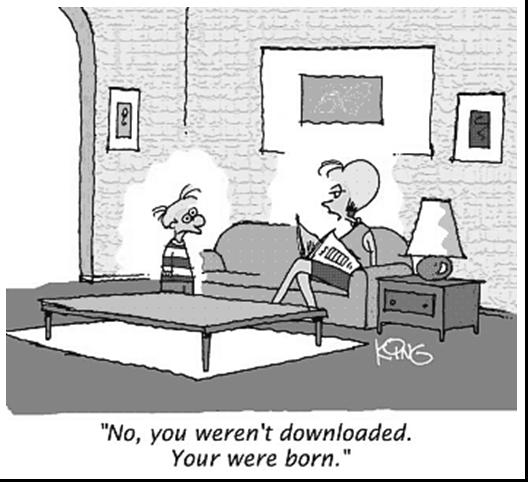
\includegraphics[width=0.85\linewidth]{template_fig1.jpg}
  \caption{[Legenda da figura de resultados]}
  \label{fig:resultados-exemplo}
\end{figure}

% =================================================================
% CAPÍTULO 8: CONCLUSÕES E CONTRIBUIÇÕES (TEMPLATE)
% Objetivo: fechar argumentos, sintetizar resultados e destacar contribuições.
% Dicas:
%  - Evite introduzir conteúdo novo; foque na síntese.
%  - Separe claramente conclusões, contribuições e limitações.
% =================================================================
\section{Conclusões e Contribuições}

[Resuma as conclusões frente aos objetivos e destaque as contribuições do trabalho.]

\subsection{Conclusões}
[Apresente as principais conclusões e impactos.]

\subsection{Contribuições}
[Detalhe contribuições teóricas, práticas e metodológicas.]

\subsection{Limitações}
[Descreva limitações e ameaças à validade.]


% =================================================================
% BIBLIOGRAFIA (thebibliography - padrão simples)
% =================================================================
% =================================================================
% BIBLIOGRAFIA
% =================================================================

\begin{thebibliography}{99}

\bibitem{ref:exemplo}
[Autor]. [Título]. [Ano]. [Local/Periódico]. [Editora/DOI/URL].

\end{thebibliography}


% Opção alternativa — BibTeX (.bib): comente a linha acima e descomente as duas abaixo.
% \bibliographystyle{sbc}
% \bibliography{bibliography/sbc-template}

\end{document}
